\graphicspath{{Kapitel/Kapitel_Vorbereitungen/Images/}}

%TODO
Kurze Einleitung was alles vorbereitet wurde.

\section{Das C.LABEL Tool}
\label{C.LABEL}
%TODO 
Beschreibung des C.Label Tools, was es kann, was in die VR übernommen werden soll und was deswegen für die weitere Auswahl an HW und Tools zu berücksichtigen ist

\section{Wahl des passenden Mediums} 
Um das Labeln von Daten, insbesondere Punktwolken, im dreidimensionalem Raum zu verwirklichen gibt es zwei wesentliche Technologien die dafür relevant erscheinen. Diese sind Augmented Reality und Virtual Reality.\\

Unter \acrfull{acr:AR} versteht man die direkte oder indirekte Sicht auf die reale, physische Welt, welche durch digitale Inhalte erweitert wird. Dies wird vor allem durch Smartphones oder \acrshort{acr:AR}-Brillen realisiert. Bei einem Smartphone hat man beispielsweise einen indirekten Blick auf die reelle Umgebung durch das Display, welches ein Live-Bild der Kamera anzeigt. Diesem Bild können nun digitale Inhalte hinzugefügt werden. Bei einer Brille (Abbildung \ref{fig:Hololens}: Microsoft Hololens \acrshort{acr:AR}-Brille) sieht man durch die Gläser direkt auf die physische Welt. Hierbei fungieren die Gläser als Display, welche in der Lage sind Holographische Objekte anzuzeigen. Dies führt zu einer, für den Benutzer, sehr immersiven Vermischung der realen und der digitalen Welt. Üblicherweise ist es bei diesen Brillen sogar möglich durch Gesten, die mittels Händen durchgeführt werden, mit den Hologrammen zu interagieren.\\

\acrfull{acr:VR} ist eine Technologie bei der spezielle \acrshort{acr:VR}-Brillen zum Einsatz kommen, welche keine Sicht mehr auf die reale Umgebung ermöglichen (Abbildung \ref{fig:Oculus}: Oculus Rift \acrshort{acr:VR}-Brille). Das Blickfeld des Menschen wird hierbei komplett von einem Display abgedeckt, das sich im Inneren der Brille befindet. So kann dem Benutzer eine komplette virtuelle Welt angezeigt werden. Mittels kompatiblen Controllern (Abbildung \ref{fig:Oculus}: Oculus Rift \acrshort{acr:VR}-Brille) kann dieser sich durch diese Welt bewegen bzw. mit ihr interagieren. Die Controller werden dabei von einem Sensor erfasst und somit können reale Bewegungen der Controller in die virtuelle Welt übersetzt werden.\\

\begin{figure}%
    \centering
    \subfloat[Microsoft Hololens \acrshort{acr:AR}-Brille]{{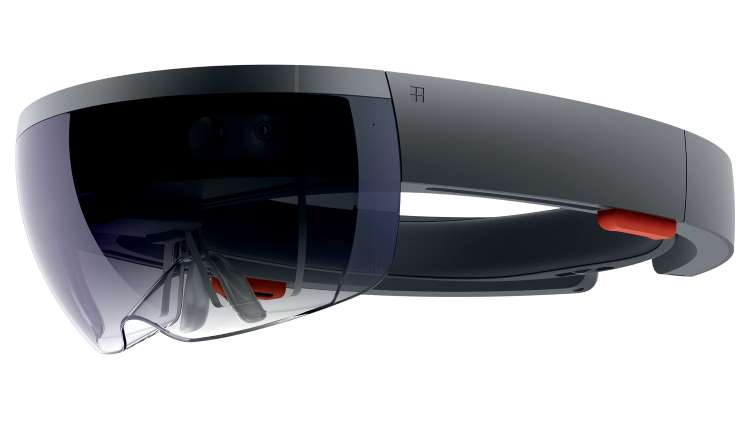
\includegraphics[width=5cm]{Hololens}\label{fig:Hololens}}}%
    \qquad
    \subfloat[Oculus Rift \acrshort{acr:VR}-Brille]{{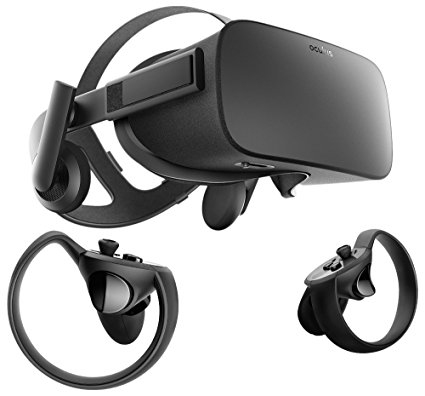
\includegraphics[width=4cm]{Oculus}\label{fig:Oculus}}}%
    \caption{Beispiel für \acrshort{acr:AR}/\acrshort{acr:VR}-Brillen}%
\end{figure}

Im folgenden Abschnitt wird auf die positiven und negativen Aspekte der beiden Technologien eingegangen. Hierbei werden vor Allem die Anforderungen für das Labeling von Punktwolken berücksichtigt, weshalb die hervorgebrachten Vor- und Nachteile eventuell für andere Anwendungsfälle nicht aussagekräftig sind.

\subsection{Eignung von \acrlong{acr:AR} und \acrlong{acr:VR} im Bezug auf 3D-Datennotation}
%TODO
\subsubsection{Eignung von \acrlong{acr:AR}}
Der, im Rahmen dieser Arbeit, entwickelte Prototyp zur 3D-Datennotation ist nicht nur als Nutzungssoftware geplant, sondern dient auch als Anschauungsmaterial, beispielsweise für Messen. Zieht man diese Tatsache in Betracht, eignet sich \acrlong{acr:AR} sehr gut für diesen Zweck. Es wirkt durch die Vermischung von realen und digitalen Inhalten sehr futuristisch. Zudem ist das direkte einblenden holographischer Inhalte, durch eine \acrshort{acr:AR}-Brille, zum Zeitpunkt der Erstellung dieser Arbeit, noch wenig verbreitet, was bei unwissenden Benutzern einen beeindruckenden Effekt hervorruft. Zum Zeitpunkt dieser Arbeit wurde die Hololens-Brille von Microsoft beispielsweise nur wenige Tausend mal verkauft, wie einem Interview von Roger Walkden, dem Verkaufsleiter der Hololens, zu entnehmen ist \cite{HololensVerkaufszahlen}. Des Weiteren bietet die \acrlong{acr:AR} Technologie viele, für zukünftige Labeling-Methoden, relevante Möglichkeiten. Den heutigen \acrshort{acr:AR}-Brillen ist es durch Tiefenkameras möglich Objekte und deren Distanzen zur Brille wahrzunehmen. Folglich könnte ein zukünftiger Ansatz sein, eine Punktwolke der Umgebung, wie sie in \ref{C.LABEL} zu sehen ist, mit einer \acrshort{acr:AR}-Brille zu erstellen. Diese kann anschließend vor Ort, in der Umgebung in der die Punktwolke erstellt wurde, gelabelt werden.\\ %TODO Dieser Ansatz könnte ausführlicher sein. 

Ein wichtiger Punkt der ebenfalls betrachtet werden muss ist die Bedienung der Brille bzw. die Interaktion mit den digital dargestellten Objekten und Informationen. Die Steuerung von \acrshort{acr:AR}-Brillen erfolgt handelsüblich über Gesten, welche man mit seiner Hand bzw. seinen Händen tätigt. Ob diese Art der Interaktion für den betrachteten Anwendungsfall passend wäre, lässt sich im Voraus schwer feststellen. Denkbar wäre, dass sich Benutzer durch intuitive Gesten, die man auch bei realen Objekten nutzen würde, schnell an die Benutzung des Tools gewöhnen würden. Andererseits könnte die Selektion der Elemente einer Punktwolke zu ungenau sein, da die Brille die Position der Hand nicht richtig interpretiert bzw. diese nicht richtig zu Position der digitalen Inhalte interpretiert. Eine genaue Einschätzung der Bedienung für solch einen Anwendungsfall kann allerdings nur gegeben werden indem man einen Labeling-Prototypen für diesen Anwendungsfall erstellt und ihn analysiert.\\  

Darüber hinaus gibt es natürlich auch Aspekte die gegen die \acrshort{acr:AR}-Technologie sprechen. Das labeln einer Punktwolke mit dieser Technik ist an einem normalen Büro-Arbeitsplatz nicht möglich, zumindest nicht in einem Maßstab in dem es sinnvoll wäre. Die holographischen Punkte kollidieren, wenn sie darauf programmiert sind, mit der Umgebung und so würde Darstellung des Umfeldmodells verfälscht werden. Selbst wenn sie das nicht wären, dann wäre die Umgebung immer noch ein Hindernis für den Benutzer, denn man möchte sich ja durch die Punktwolke bewegen. Des Weiteren sind bei \acrshort{acr:AR}-Brillen die vorherrschenden Lichtbedingungen ein großer Faktor, welche die Funktionalität gewisser Anwendungsfälle beeinflussen können. Wird beispielsweise eine Lichtquelle von einem Objekt zu sehr reflektiert, kann dieses von der Tiefenkamera der Brille nicht mehr richtig erfasst werden. Somit würde das Umfeldmodell nicht mehr mit der Realität übereinstimmen. Für die Entwicklung der gewünschten Methode zur 3D-Datennotation ist es ebenfalls hinderlich, dass es, zum Zeitpunkt der Erstellung dieser Arbeit, wenig Dokumentationen und Hilfestellungen, zum Beispiel in Entwicklerforen, gibt. Dies ist jedoch üblich für Technologien, die noch nicht lange auf dem Markt sind. Zu guter Letzt ist noch der finanzielle Faktor zu berücksichtigen. Durch die Aktualität der Technologie ist diese auch sehr teuer. Der Preis für eine \acrshort{acr:AR}-Brille kann dabei den Betrag von 5.000 Euro überschreiten, wie im  Abschnitt \ref{ARVergleich} näher erläutert wird.    

\subsubsection{Eignung von \acrlong{acr:VR}} 

Die \acrlong{acr:VR} Technologie bietet den großen Vorteil, beliebig große Räume virtuell begehbar zu machen, ohne sich in der realen Welt selbst bewegen zu müssen. Dies ermöglicht die Bewegung durch Punktwolken, die im dreidimensionalen Raum dargestellt sind, an jedem üblichen Arbeitsplatz eines Büros. Des weiteren wirkt die Steuerung der \acrshort{acr:VR}-Brillen mittels den zugehörigen Controllern zum teil sehr ausgereift. Die Positions- und Bewegungserkennung des Benutzers wird als \glqq äußerst präzise\grqq beschrieben \cite{ControllerTest}. Dies ist sehr wichtig um die Handhabung der Anwendung für den späteren Endnutzer so angenehm wie möglich zu machen. Für die Entwicklung von \acrshort{acr:VR}-Applikationen selbst ist zu sagen, dass es mittlerweile sehr Umfassende Dokumentationen, Anleitungen und Beiträge zu den jeweiligen Plattformen und \glspl{acr:SDK} gibt. Dies hängt damit zusammen, dass sich die \acrlong{acr:VR} Technologie schon etwas länger auf dem Markt befindet und die Zahl der Entwickler für \acrshort{acr:VR}-Applikationen stetig steigt. Dies ist vermutlich nicht zuletzt der Tatsache zu verdanken, dass die Preise für \acrshort{acr:VR}-Brillen gesunken sind. Wie im späteren, ausführlicher beschreibenden, Abschnitt \ref{ARVergleich} gezeigt, beträgt der aktuelle Preis einer Oculus Rift 449 Euro. Sowohl die zahlreichen Informationen für Entwickler als auch der niedrige Preis der Hardware sprechen, neben den zuvor genannten Aspekten, für Wahl von \acrlong{acr:VR} als Plattform für die Entwicklung von 3D-Labeling.\\

Was mit der \acrshort{acr:VR}-Technologie nur schwer möglich ist, ist die physische Begehung einer, zu labelnden, Punktwolke. Zwar bietet die Technik die Möglichkeit durch zusätzliche Sensoren die Bewegungen des Benutzers in die virtuelle Welt zu übersetzen, jedoch funktioniert dies nur auf begrenztem Raum und ist unmöglich an einem üblichen Büro-Arbeitsplatz möglich. Der reale begehbare Raum muss nämlich beispielsweise durch Sensoren abgesteckt werden. Ein weiter Negativaspekt ist, dass viele Benutzer von \acrshort{acr:VR}-Brillen über Übelkeit klagen. In manchen Tests sind es mehr als 50 Prozent aller Teilnehmer, vor allem wenn es sich um Frauen handelt \cite{VRSickness}. 


\subsection{\acrshort{acr:AR}-Brillen im Vergleich}
\label{ARVergleich}
%TODO 
Vor- und Nachteile beider AR-Brillen im Bezug auf die Anforderungen

\subsection{\acrshort{acr:VR}-Brillen im Vergleich}
%TODO 
Vor- und Nachteile beider AR-Brillen im Bezug auf die Anforderungen

\subsection{Erläuterung der Entscheidung}
%TODO 
Welche Kriterien sind am wichtigsten und warum?

\section{Wahl des passenden Rechners}
%TODO

\section{Wahl der passenden Entwicklungsplattform}
%TODO 
test für pi \gls{symb:Pi}
Welche gibt es? warum keine anderen?
\subsection{\acrlong{acr:UE}}
%TODO
Full\acrfull{acr:UE}   short\acrshort{acr:UE}
Was kann die Unity Engine? Aufzählung von Fakten etc.
Vor und nachteile
\subsection{\acrlong{acr:UE4}}
%TODO
Was kann die Unreal Engine 4? Aufzählung von Fakten etc.
Vor und nachteile

\subsection{Erläuterung der Entscheidung}
%TODO 
Erläuterung was besser wäre -> beide gut
=> Beispielprojekt










